\documentclass[main.tex]{subfiles}
\begin{document}

\marginpar{Tuesday\\ 2021-11-30}

We want to introduce some thermodynamic quantities for the plasma. 

Let us start from the MHD equations: 
%
\begin{align}
\pdv{\rho }{t} + \vec{\nabla} \cdot (\rho \vec{u}) &=  0 \\
\rho \dv{\vec{u}}{t} + \rho \vec{u} \cdot \vec{\nabla} \vec{u} &= - \vec{\nabla} P + \frac{1}{4 \pi } \qty(\vec{\nabla} \times \vec{B}) \times \vec{B}
\,.
\end{align}

We introduce the additional assumption that the plasma is isentropic: 
%
\begin{align}
\qty[ \pdv{}{t} + \vec{u} \cdot \vec{\nabla}] P \rho^{-\gamma } = 0
\,,
\end{align}
%
as well as the magnetic field equations: 
%
\begin{align}
\vec{\nabla} \cdot \vec{B} &= 0  \\
\pdv{\vec{B}}{t} + \vec{\nabla} \times \qty(\vec{u} \times \vec{B}) &= 0
\,.
\end{align}

We can always put ourselves in a frame which is at equilibrium: \(\vec{u} = 0\), which we then perturb with \(\delta \vec{u}\). 

Then, we move to Fourier space and do first-order perturbation theory: we find 
%
\begin{align}
-i \omega \delta \rho + i \vec{k} \cdot \delta \vec{u} \rho &= 0  
\,.
\end{align}

The entropy equation becomes 
%
\begin{align}
\pdv{P }{t} \rho^{-\gamma } - \gamma \rho^{-\gamma -1} P \pdv{\rho }{t} &= 0  \\
- i \omega \delta P + \gamma \rho^{-\gamma -1} P i \omega \delta \rho  &= 0  \\
- i \omega \delta P + \gamma \frac{P}{\rho } i \omega \delta \rho &= 0  \\
\pdv{ \delta P}{ \delta \rho } &= \gamma \frac{P}{\rho } = c_s^2
\,,
\end{align}
%
so we have found acoustic perturbations by allowing the plasma to be compressible. 

The no-monopoles equation becomes \(i \vec{k} \cdot \delta \vec{B} = 0\); while the last one can only be perturbed like 
%
\begin{align}
- i \omega \delta \vec{B} &= i \vec{k} \times \qty( \delta \vec{u} \times \vec{B})  \\
\delta \vec{B} &= - \frac{\vec{k}}{\omega } \times \qty( \delta \vec{u} \times \vec{B}) 
\,.
\end{align}

The momentum conservation law becomes 
%
\begin{align}
- i \omega  \rho \delta \vec{u}  &= - i \vec{k} \delta P + \frac{i \vec{k}}{4 \pi } \times \delta \vec{B} \times \vec{B}_0   \\
&= - i \vec{k} c_s^2 \delta \rho - \frac{i}{4 \pi \omega } \vec{k} \times \qty(\vec{k} \times \qty( \delta \vec{u} \times \vec{B}_0)) \times \vec{B}_0  \\
- i \omega \rho \delta \vec{u} &= 
- i \vec{k} c_s^2 \frac{\rho}{\omega } \vec{k} \cdot \delta \vec{u} - \frac{i}{4 \pi \omega } \vec{k} \times \qty(\vec{k} \times \qty( \delta \vec{u} \times \vec{B}_0)) \times \vec{B}_0
\marginnote{Used \(\delta \rho = (\rho / \omega ) \vec{k} \cdot \delta \vec{u}\).} 
\,.
\end{align}

This is now all written in terms of \(\delta \vec{u}\), and it contains all MHD perturbations. 

Let us look at some specific cases: first, assume \(\vec{B}_0 = B_0 \hat{z}\), and that \(\vec{k}\) is parallel to it, so \(\vec{k} = k \hat{z}\). 

The cross product term reads:
%
\begin{align}
\delta \vec{u} \times \vec{B}_0 &= \left[\begin{array}{c}
\delta u_y B_0  \\ 
- \delta u_x B_0  \\ 
0
\end{array}\right]  \\
\vec{k} \times (\delta \vec{u} \times \vec{B}_0) &= \left[\begin{array}{c}
k \delta u_x B_0  \\ 
k \delta u_y B_0  \\ 
0
\end{array}\right] \\
\vec{k} \times \qty(\vec{k} \times (\delta \vec{u} \times \vec{B}_0)) &= \left[\begin{array}{c}
-k^2 \delta u_y B_0  \\ 
k^2 \delta u_x B_0  \\ 
0
\end{array}\right] 
\\
\qty[\vec{k} \times \qty(\vec{k} \times (\delta \vec{u} \times \vec{B}_0))]\times \vec{B}_0 &= \left[\begin{array}{c}
k^2 \delta u_x B_0^2  \\ 
k^2 \delta u_y B_0^2s  \\ 
0
\end{array}\right] 
\,.
\end{align}

The equation is therefore 
%
\begin{align}
- i \omega \rho \left[\begin{array}{c}
\delta u_x \\ 
\delta u_y \\ 
\delta u_z
\end{array}\right]
&= -i c_s^2 \frac{\rho}{\omega } 
\left[\begin{array}{c}
0 \\ 
0 \\ 
k
\end{array}\right] k \delta u_z 
- \frac{i}{4 \pi \omega } 
\left[\begin{array}{c}
k^2 \delta u_x B_0^2  \\ 
k^2 \delta u_y B_0^2s  \\ 
0
\end{array}\right] 
\,,
\end{align}
%
where we can see that the perpendicular and parallel modes are decoupled: the \(z\) mode reads 
%
\begin{align}
\omega \rho \delta u_z = c_s^2 \frac{\rho}{\omega } k^2 \delta u_z \implies \omega^2 = k^2 c_s^2
\,,
\end{align}
%
therefore the \emph{longitudinal} modes are \emph{sound waves}! 
For those modes the magnetic field is irrelevant since \(\delta \vec{u} \times \vec{B}_0 = 0\). 

What about the other directions? We find 
%
\begin{align}
\omega \rho = \frac{k^2B_0^2}{4 \pi \omega } \implies \omega^2 = k^2 \frac{B_0^2}{4 \pi \rho } = k^2 v_A^2
\,,
\end{align}
%
so these are Alfén waves. 
This tells us that these are \emph{transverse} waves, but still propagating \emph{along} the magnetic field. 

What is the magnetic field perturbation? 
%
\begin{align}
\delta \vec{B} &= - \frac{1}{\omega } \vec{k} \times 
\qty( \delta \vec{u} \times \vec{B}_0)  \\
&= - \frac{1}{\omega } \left[\begin{array}{c}
k B_0 \delta u_x \\ 
k B_0 \delta u_y \\ 
0
\end{array}\right]
\,,
\end{align}
%
which means that the magnetic field is also only oscillating along the \(x\) and \(y\) directions. 

We can also compute the induced electric field: 
%
\begin{align}
\delta \vec{E} = - \frac{1}{c} \delta \vec{u} \times \vec{B}_0 = \left[\begin{array}{c}
 \delta u_y B_0 / c \\ 
\delta u_x B_0 / c \\ 
0
\end{array}\right]
\,.
\end{align}

The perturbations in the magnetic field, \(\sim B_0  \delta u / v_A\) are \emph{larger} than the ones in the electric field, \(\sim B_0 \delta u /c\)! 
This can be also checked when looking at the Lorentz force expression. 

Let us then look at the perpendicular modes: \(\vec{k} \perp B_0 \), specifically \(\vec{k} = k \hat{x}\). 

%
\begin{align}
\delta \vec{u} \times \vec{B}_0 &= \left[\begin{array}{c}
\delta u_y B_0  \\ 
- \delta u_x B_0  \\ 
0
\end{array}\right]  \\
\vec{k} \times (\delta \vec{u} \times \vec{B}_0) &= 
\left[\begin{array}{c}
0 \\ 
0 \\ 
- k \delta u_x B_0 
\end{array}\right] \\
\vec{k} \times \qty(\vec{k} \times (\delta \vec{u} \times \vec{B}_0)) &= 
\left[\begin{array}{c}
0 \\ 
k^2 \delta u_x B_0  \\ 
0
\end{array}\right] \\
\qty[\vec{k} \times \qty(\vec{k} \times (\delta \vec{u} \times \vec{B}_0))]\times \vec{B}_0 &= 
\left[\begin{array}{c}
k^2 \delta u_x B_0^2 \\ 
0  \\ 
0
\end{array}\right]
\,.
\end{align}

Plugging this into the equation yields 
%
\begin{align}
- i \omega \rho \left[\begin{array}{c}
\delta u_x \\ 
\delta u_y \\ 
\delta u_z
\end{array}\right]
= - i \left[\begin{array}{c}
k \\ 
0 \\ 
0
\end{array}\right]
c_s^2 \frac{\rho}{\omega } k \delta u_x
- \frac{i}{4 \pi \omega } \left[\begin{array}{c}
k^2 B_0^2 \delta u_x \\ 
0 \\ 
0
\end{array}\right]
\,,
\end{align}
%
which means that the only nonzero component, along \(x\), reads 
%
\begin{align}
\omega^2 = \qty(c_s^2 + \frac{B_0^2}{4 \pi \rho })k^2 = \qty(c_s^2 + v_A^2) k^2
\,,
\end{align}
%
which is commonly called a ``fast'' \textbf{magnetosonic mode}. 

For the rest of the course we will focus on the Alfvén modes. 

\section{High energy particles}

We start by assuming we already have a non-thermal, high energy particle. 

The momentum of the particle is \(\vec{p} = m \vec{v} \gamma \), while the field is \(\vec{B}_0 = B_0 \hat{z}\). 

The energy of this particle will not change under the action of the magnetic field; the Lorentz force's action means we will have 
%
\begin{align}
\dv{\vec{p}}{t} = q \frac{\vec{v}}{c} \vec{B}_0
\,,
\end{align}
%
therefore 
%
\begin{align}
m \gamma \dv{v_x}{t} = q \frac{v_y}{c} B_0 \marginnote{\(\gamma \) is a constant: the energy cannot change.}\\
m \gamma \dv{v_y}{t} = - q \frac{v_x}{c} B_0 \\
\dv{v_z}{t} = 0
\,.
\end{align}

Putting these together we get 
%
\begin{align}
\qty(\frac{m \gamma }{q B_0 })^2 \dv[2]{v_x}{t} &= - v_x  \\
\dv[2]{v_x}{t} &= - \Omega^2 v_x
\,. 
\end{align}

If \(\gamma = 1\), this is the cyclotron frequency; otherwise, it is just \(\Omega = q B_0 / (m c \gamma )\). 

If \(\mu \) is the cosine of the angle between the initial velocity and the magnetic field, the solution will read 
%
\begin{align}
v_x (t) &= v_0 (1 - \mu^2)^{1/2} \cos( \Omega t) \\
v_y (t) &= v_0 (1 - \mu^2)^{1/2} \sin( \Omega t)  \\
v_z (t) &= v_0 \mu 
\,.
\end{align}

What happens if this trajectory is perturbed, say, by an Alfvén wave? 
The field will now be \(\vec{B} = \vec{B}_0 + \delta \vec{B}\), and we will work to first order in \(\delta \vec{B}\). 

Let us assume one of these two things: 
\begin{enumerate}
    \item we sit in a reference frame moving with the waves, so that the electric field perturbation vanishes;
    \item we decide to neglect the electric field since we know its effect to be small.
\end{enumerate}

There is a subtle difference between the two. 

We assume that the polarization of the electric field perturbation is circular: \(\delta E_y = \pm i \delta E_x\), so that \(\delta B_x = \mp \delta B_y\). 

We take 
%
\begin{align}
\delta B_y &= \exp(i \qty(kz - \omega t + \varphi )) 
\,,
\end{align}
%
where we insert an arbitrary initial phase we will later average over. 

If we take the real part of the perturbation, we get 
%
\begin{align}
\delta B_x &= \pm \sin(kz - \omega t + \varphi ) \\ 
\delta B_y &= \pm \cos(kz - \omega t + \varphi ) 
\,.
\end{align}

This is an Alfvén wave, so \(\omega = k v_A\). 

If we assume that the electric field is negligible, the equations of motion for the particle will be modified as 
%
\begin{align}
\dv{\vec{p}}{t} = q \frac{\vec{v}}{c} \times \qty(\vec{B}_0 + \delta \vec{B})  &= \frac{q}{c} \left[\begin{array}{ccc}
\hat{x}  & \hat{y} & \hat{z} \\ 
v_x & v_y & v_z \\ 
\delta B_x & \delta B_y & B_0 
\end{array}\right]  \\
m \gamma \dv{}{t} \left[\begin{array}{c}
v_x \\ 
v_y \\ 
v_z
\end{array}\right]
&= 
\left[\begin{array}{c}
v_y B_0 - v_z \delta B_y \\ 
- v_x B_0 + \delta B_x v_z \\ 
v_x \delta B_y - v_y \delta B_x
\end{array}\right]
\,.
\end{align}

Looking at the \(z\) component, we see that the perturbation changes \(v_z\), but \(v_0 \) is constant, so the pitch angle \(\mu \) must be changeing. 

Why is this relevant? We know that spallation must occur, so the cosmic rays must remain in the galaxy for a while. 
This can be a mechanism to explain that. 

We focus on the \(z\) equation: 
%
\begin{align}
m \gamma \dv{v_z}{ t} &= 
\frac{q}{c} \delta B v_0 (1 - \mu^2)^{1/2} 
\qty(
\cos(\Omega t) \cos( k z  - \omega t + \varphi ) 
\pm 
\sin(\Omega  t) \sin(k z - \omega t + \varphi )  )
\\
m \gamma v_0 \dv{\mu }{t} &= \frac{q \delta B}{mc \gamma } v_0 (1 - \mu^2)^{1/2}  
\qty(\cos(\Omega t) \cos(k z - \omega t + \varphi ) \pm \sin(\Omega t) \sin(kz - \omega t + \varphi ))  \\
\dv{\mu }{t}&= \frac{q \delta B}{mc \gamma } v_0 (1 - \mu^2)^{1/2}
\cos(\Omega t \mp kz \pm \omega t \mp \varphi ) 
\marginnote{Used some ugly prostapheresis formulae.}
\,.
\end{align}

Now, however, \(kz \approx k v_0 \mu t\); however, \(\omega t \approx k v_A t\), so unless \(\mu \lesssim v_A /c \) the latter is negligible. 

In normal conditions, \(v_A \ll v_0 \sim c\), and this is a requirement of the order of \(\num{e-6}\). 

The falsifying example is a particle moving basically moving in a circle without any \(z\) component to its velocity, but this is very unlikely. 

The wave, for the relativistic particle, is basically stationary. 

So, 
%
\begin{align}
\dv{\mu }{t} = \frac{q \delta B}{mc \gamma } (1 - \mu )^{1/2} \cos(\Omega t \mp kv_0 \mu t \mp \varphi ) 
\,.
\end{align}

To find out what the effect of this is over a long period of time we need to integrate. 

The mean value of the cosine vanishes, however, we can have a diffusion-like process. 
On average, \(\expval{ \Delta \mu }= 0\), but we might want to compute \(\expval{ \Delta \mu \Delta \mu }\):
this will be 
%
\begin{align}
\expval{\Delta \mu  \Delta \mu } = \qty(\frac{q \delta B}{mc \gamma })^2 (1 - \mu^2) \int_0^{T} \dd{t} \int_0^{T} \dd{t'} 
\cos ( (\Omega \mp v_0 k \mu ) t \mp \varphi )
\cos ( (\Omega \mp v_0 k \mu ) t' \mp \varphi )
\,,
\end{align}
%
where the first thing we want to do is to also take an average over \(\varphi \): 
%
\begin{align}
\expval{\Delta \mu  \Delta \mu } &= \qty(\frac{q \delta B}{mc \gamma })^2 (1 - \mu^2) \frac{1}{2} \int_0^{T} \dd{t} \int_0^{T} \dd{t'} 
\cos ( (\Omega \mp v_0 k \mu ) (t-t'))  \\
&= \qty(\frac{q \delta B}{mc \gamma }) (1 - \mu^2) \frac{2 \pi }{2} T \delta (\Omega \mp v_0 k \mu )  \\
&= \qty(\frac{q \delta B}{mc \gamma }) (1 - \mu^2) \pi T \delta (k \mp \frac{\Omega}{v_0 \mu })
\,,
\end{align}
%
so we do indeed get a diffusion-like motion with variance \(\sim T\). 

However, this is only the case if 
%
\begin{align}
k = \pm \frac{\Omega }{v_0 \mu } = \pm \frac{1}{r_L \mu }
\,.
\end{align}

So, only if the wave is \emph{resonant} with the Larmor radius then its pitch angle \emph{diffuses}. 

This remains quite close to being true even if the assumption of small \(\delta B\) is relaxed. 

More specifically, 
%
\begin{align}
k = \pm \frac{\text{sign}\ q}{\abs{r_L} \mu }
\,.
\end{align}

It is customary to introduce a \emph{diffusion coefficient}: 
%
\begin{align}
D_{\mu \mu } &= \frac{1}{2} \expval{\frac{\Delta \mu \Delta \mu }{\Delta t}} 
= \frac{1}{2} \qty(\frac{q \delta B}{mc \gamma })^2 (1 - \mu^2)  \frac{\pi}{v_0 \mu } \delta (k \mp \frac{\Omega }{v_0 \mu } )  \\
&= \qty( \frac{q B_0 }{mc \gamma })^2 \frac{ \delta B^2}{B_0^2} (1 - \mu^2) \frac{\pi }{2 v_0 \mu } \delta (k \mp \frac{\Omega}{\mu v_0 }) 
\,.
\end{align}

This is useful since in general \(\delta B\) will depend on the scale: there are no monochromatic Alfvén waves in nature. 
Therefore, 
%
\begin{align}
D_{\mu \mu } &= \Omega^2 (1 - \mu^2) \frac{\pi}{2 v_0 \mu } \int \dd{k} \frac{ \delta B^2 (k)}{B_0^2} \delta (k \mp \frac{\Omega}{v_0 \mu })  \\
&= \Omega^2 (1 - \mu^2) \frac{\pi }{2 v_0 \mu } \frac{ \delta B^2 (k _{\text{res}})}{B_0^2}  \\
&= \frac{\pi}{2} \Omega (1 - \mu^2) k _{\text{res}} F(k _{\text{res}})
\,,
\end{align}

where 
%
\begin{align}
F (k _{\text{res}}) = \frac{1}{B_0^2} \delta B^2 (k _{\text{res}})
\,.
\end{align}

We can also compute \(D_{\theta \theta }\): 
%
\begin{align}
D_{\theta \theta } = \frac{\pi}{2} \Omega k _{\text{res}} F(k _{\text{res}})
\,.
\end{align}

How long does it take to have a diffusion by, say, 1 radian? it will be 
%
\begin{align}
\tau \sim \frac{1}{D_{\theta \theta }} \sim \frac{1}{\Omega k _{\text{res}} F(k _{\text{res}})}
\,.
\end{align}

\begin{figure}[ht]
\centering
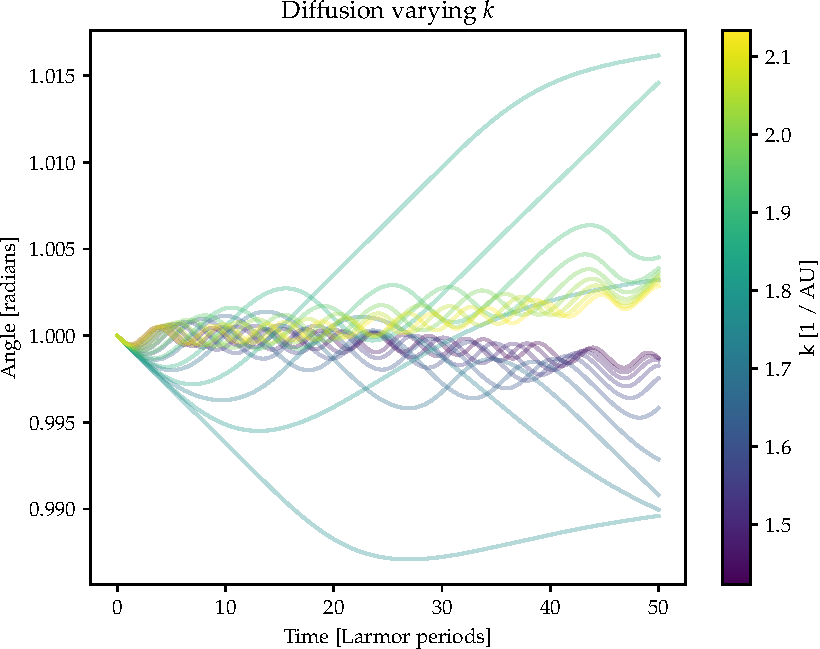
\includegraphics[width=\textwidth]{figures/diffusion_over_time}
\caption{Diffusion over time. The evolution is shown for a relativistic proton with \(\gamma = 10\), moving across a field 
\(B_0 = \SI{2}{\micro\gauss}\) 
with a perturbation \(\delta B = \num{e-4} B_0 \), with the \(+\) circular polarization (i.\ e.\ all the \(\pm\) become \(+\), all the \(\mp\) become \(-\)). A white mark on the wavenumber scale marks \(k = \Omega v_0 \cos \theta \), at which the ``resonance'' happens.}
\label{fig:diffusion_over_time}
\end{figure}

\begin{figure}[ht]
\centering
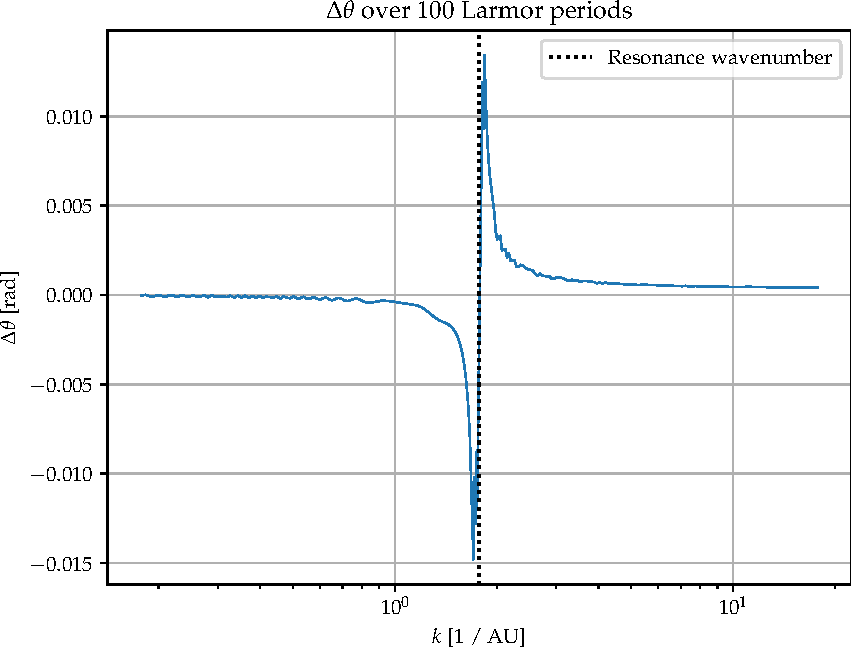
\includegraphics[width=\textwidth]{figures/final_point_variation}
\caption{\(\Delta \theta \) corresponding to the end of the integrated curves in figure \ref{fig:diffusion_over_time}.}
\label{fig:final_point_variation}
\end{figure}

\todo[inline]{There seems to be a high tail at high \(k\)!}

\end{document}
